\chapter{Protocoles et mécanismes d'Internet}

\section{Présentation du protocole HTTP}
HTTP (HyperText Transport Protocol) \cite{Obo_CNP3} est un protocole qui fournit les fondations du World Wide Web, il repose sur le modèle client-serveur dans lequel le client envoie une requête et le serveur retourne une réponse. Il est décrit par la RFC 2616 \cite{IETF_RFC2616}.

Les requêtes HTTP se composent de trois parties :
\begin{enumerate}
	\item Une ligne de requête (qui contient notamment une URI)
	\item Des entêtes (qui contiennent des paramètres pour la requête)
	\item Le corps de la requête (optionnel)
	\newline
\end{enumerate}

Lorsqu'un utilisateur clique sur un lien hypertexte via son navigateur, celui-ci se connecte à un serveur identifié par l'URI "Uniform Resource Identifier" présent dans ce lien. Le navigateur envoie alors une requête à laquelle le serveur répond puis le navigateur se déconnecte du serveur. On considère que la requête est sans état car à chaque fois que le navigateur crée une connexion pour une requête, le serveur la traite comme si c'était la première ; les requêtes sont donc indépendantes.

Les réponses HTTP se composent également de trois parties :
\begin{enumerate}
	\item Une ligne de statut (qui indique si la requête est réussie ou pas)
	\item Des entêtes (qui contiennent des informations sur la réponse)
	\item Le corps de la réponse
	\newline
\end{enumerate}

Il fallait trouver une solution afin d'avoir la possibilité de garder une certaine quantité d'informations entre des requêtes successives. En effet, si le serveur est dans l'incapacité de se souvenir de ce que le client a fait auparavant, il est par exemple impossible de développer un site de e-commerce étant donné que celui-ci ne sauvegarderait pas la liste des articles du panier virtuel.

Une première solution consistait à forcer l'authentification du client (comme pour FTP) mais ce n'est pas toujours nécessaire ou applicable sur tous les sites web.

Une seconde solution était d'utiliser les différents types d'entêtes \emph{Accept-*}. Par exemple, un client aurait pu utiliser l'entête \emph{Accept-Language} pour indiquer la langue dans laquelle il voulait visiter le site. Cependant, cela fournit des possibilités assez limitées car cet entête est réglé par le navigateur et le client aurait été dans l'impossibilité d'indiquer une langue différente pour chaque site visité sans devoir effectuer une manipulation conséquente.

Une autre solution, qui est la plus largement adoptée, est l'utilisation d'un cookie HTTP. Elle est expliquée plus en détail dans la section suivante.
\newline

Des exemples de requête et réponse HTTP sont disponibles dans la \autoref{http_request_example}.


%%%%%%%%%%%%%%%%%%%%%%%%%%%%%%
\section{Cookies}
Une première description informelle sur les cookies a été publiée sur le site web de Netscape Communications. Le processus de standardisation des cookies a commencé en avril 1995 sur la liste de diffusion [www-talk], ensuite, l'IETF (Internet Engineering Task Force) a entrepris d'écrire un standard pour les cookies \cite{Kristol:2001:HCS:502152.502153}. C'est ainsi que la première RFC (RFC 2109) sur les cookies est parue en février 1997 \cite{IETF_RFC2109}, rendue obsolète en octobre 2000 par la RFC 2965 \cite{IETF_RFC2965}. Elle a également été remplacée, par la RFC 6265 en avril 2011 \cite{IETF_RFC6265}, qui est toujours d'application en ce jour et constitue la référence en ce qui concerne les cookies. Il est intéressant de noter qu'une section dédiée à la vie privée (section 7) est présente dans cette dernière RFC, ce qui constitue une nouveauté.
\newline

Un cookie est un petit fichier stocké en clair sur le disque dur de l'utilisateur par le navigateur. Il fait le lien entre la session de l'utilisateur et les données enregistrées par le site web (dans une base de données par exemple). Les cookies sont transmis dans les entêtes des requêtes et des réponses HTTP \cite{IETF_RFC6265}. Notez que certains navigateurs actuels enregistrent désormais ces cookies dans une base de données. C'est notamment le cas pour Firefox 3 qui enregistre ses cookies dans une base de données SQLite.
\newline

Dans sa réponse à une requête, un serveur peut envoyer des informations arbitraires (le cookie) dans un entête \textit{Set-Cookie}. Cette information peut contenir n'importe quoi et c'est elle qui permet au serveur de continuer là où il en était. Il peut s'agir d'un identifiant relatif à l'utilisateur, une clé dans une base de données,...
Le serveur peut ajouter des attributs afin de configurer les cookies (sections 5.2.1 à 5.2.6 de la RFC 6265) \cite{IETF_RFC6265} :

\begin{itemize}
	\item Expires et Max-Age : date d'expiration
	\item Domain : domaine
	\item Path : chemin
	\item Secure et HttpOnly : type de connexion
	\newline
\end{itemize}

Habituellement, le client est coopératif et renvoie l'information du cookie qui est stocké par le navigateur. Dans chaque requête ultérieure qu'il fait vers le serveur, le client indique cette information dans un entête \textit{Cookie}. Le serveur peut choisir de renvoyer un nouveau cookie dans ses réponses, ce qui remplacera automatiquement l'ancien cookie.
\newline

Il y a un contrat implicite entre le client et le serveur : ce dernier repose sur le client afin de sauvegarder son état. Le serveur compte sur le client pour lui retourner son état lors de la prochaine requête. Un cookie est donc une donnée que le serveur et le client se renvoient l'un et l'autre. La quantité d'informations est généralement petite et son contenu est à la discrétion du serveur. En effet, la plupart du temps, analyser le contenu du cookie ne révèle ni à quoi il est destiné ni la valeur qu'il représente.


%%%%%%%%%%%%%%%%%%%%%%%%%%%%%%
\section{Cache}
Dans le domaine informatique, un cache permet de garder une copie locale d'un élément afin de répondre rapidement à une requête. Au lieu de récupérer l'élément, le cache renvoie sa copie, ce qui permet de réduire sensiblement le temps de réponse.\\
Le principe de cache sur le protocole HTTP est défini dans la RFC 2616 \cite{IETF_RFC2616} (sections 13 et 14). Les mécanismes de cache peuvent être implémentés à différents niveaux :
\begin{itemize}
  \item sur le réseau qui délivre le contenu d'un site web (ex. : un CDN - "Content Delivery Network")
  \item sur l'application qui gère et affiche le contenu d'un site web (ex. : un CMS - "Content Management System")
  \item sur le serveur qui héberge le site web (ex. : Apache)
  \item via le navigateur Web du client qui stocke les fichiers sur le disque dur
  \newline
\end{itemize}

Lorsque l'on navigue sur Internet, le cache du navigateur enregistre certaines ressources (images, feuilles de style, fichiers JavaScript, etc.) afin de ne pas devoir les recharger depuis le serveur lors des visites ultérieures. Par ailleurs, les administrateurs d'un site web peuvent paramétrer la mise en cache de certains éléments grâce à l'entête \textit{Cache-Control}. Celui-ci est utilisé pour spécifier des directives qui doivent être respectées par tous les mécanismes de cache le long de la chaîne requête-réponse. Grâce à ces directives, il est possible de spécifier explicitement pour chaque fichier comment il doit être traité vis-à-vis de la mise en cache \cite{IETF_RFC2616} :
\begin{multicols}{2}
\begin{itemize}
  \item public
  \item private
  \item no-cache
  \item no-store
  \item no-transform
  \item must-revalidate
  \item proxy-revalidate
  \item max-age
  \item s-maxage
  \item cache-extension
\end{itemize}
\end{multicols}

Ces directives de réponse HTTP permettent notamment d'autoriser (ou d'empêcher) la mise en cache d'un fichier, d'empêcher la mise en cache partagé ou encore, de préciser une date d'expiration à partir de laquelle le fichier présent en cache devra être revalidé.


%%%%%%%%%%%%%%%%%%%%%%%%%%%%%%
\section{Exemple de requête et réponse HTTP}
\label{http_request_example}
Voici une requête HTTP vers le site web \textit{distrowatch.com} :

\begin{singlespacing}
\lstinputlisting{examples/http_request1_distrowatch}
\end{singlespacing}
Note : aucune visite vers ce site n'a été faite auparavant.
\newline

Et la réponse HTTP associée :

\begin{singlespacing}
\lstinputlisting{examples/http_response1_distrowatch}
\end{singlespacing}
A la ligne 9, l'on peut voir un entête \textit{Set-Cookie}. Un cookie dont le nom est \textit{"NewLastSeen"} est donc créé avec la valeur "8407". Lors d'une prochaine visite sur le site, ce cookie sera alors renvoyé automatiquement dans la requête HTTP par le navigateur.\\
On peut également voir un entête \textit{Cache-Control} à la ligne 7.
\newline

Voici maintenant une seconde requête vers le même site lors de la même session. L'on peut remarquer que le navigateur envoie le cookie enregistré précédemment car la requête HTTP contient maintenant un entête \textit{Cookie} visible à la ligne 7 qui n'était pas présent dans la première requête :

\begin{singlespacing}
\lstinputlisting{examples/http_request2_distrowatch}
\end{singlespacing}

Quant à la réponse HTTP, elle reste identique.
\newline

Dans la seconde requête, l'on peut voir que le navigateur envoie 5 cookies alors qu'un seul n'a été enregistré via la réponse HTTP analysée auparavant.\\
Ceci s'explique par le fait que les cookies \textit{\_\_utmX} proviennent de Google Analytics \cite{Google_Analytics_cookies} et servent à analyser la navigation des visiteurs du site.
\newline

Il n'est pas nécessaire d'analyser les requêtes échangées pour voir les cookies envoyés : si l'on regarde dans les préférences du navigateur, on peut remarquer que 4 cookies sont présents pour l'hôte \textit{distrowatch.com} (\autoref{cookies_distrowatch}). Le cookie \textit{\_\_utmc} n'apparaît plus car il a été supprimé à la fin de sa session de navigation (suite à sa date d'expiration, voir \autoref{google_analytics}) et que la capture d'écran a été effectuée lors d'une session ultérieure.

\begin{figure}[h]
	\centering
	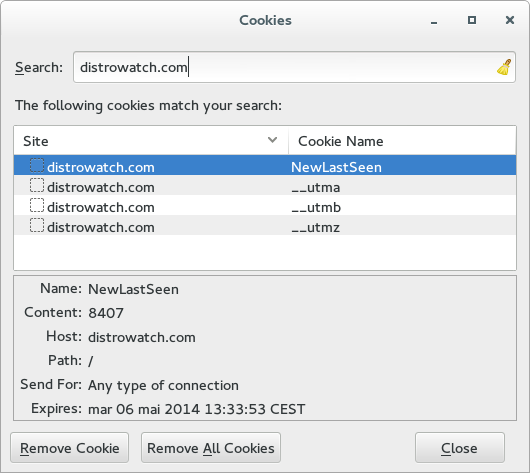
\includegraphics[scale=0.7]{figures/cookies_distrowatch.png}
	\caption{\label{cookies_distrowatch}Les cookies enregistrés pour l'hôte \textit{distrowatch.com} dans Firefox.}
\end{figure}


%%%%%%%%%%%%%%%%%%%%%%%%%%%%%%
\section{Comment le Web est-il censé fonctionner ?}
Lors du chargement d'une page web, le navigateur effectue de multiples connexions afin de récupérer l'ensemble des ressources de la page. Aux débuts du World Wide Web, toutes les ressources d'une page appartenaient généralement à une même personne/groupe. A l'heure actuelle, la situation a fortement changé : il est fréquent de voir des ressources chargées depuis des domaines tiers (régies publicitaires, CDN,...). Le navigateur effectue donc des connexions vers des serveurs différents (cela permet notamment de passer outre la limitation du nombre de connexions HTTP vers un même domaine \cite{IETF_RFC2616}) mais en contrepartie, cela permet aux serveurs en question d'enregistrer des données sur le client suite aux requêtes qu'il effectue.


%%%%%%%%%%%%%%%%%%%%%%%%%%%%%%
\section{Principe de même origine}
Le principe de même origine (\textit{same-origin principle}) peut être déclaré comme suit : "\textit{seul le site qui enregistre des données dans le navigateur peut lire ou modifier ces données plus tard}" \cite{Jackson:2006:PBS:1135777.1135884}. Son but est d'isoler des sites en respectant leur capacité à lire ou modifier l'état du navigateur. Cela permet à un utilisateur de naviguer comme si chaque site et session étaient complètement indépendants.
\newline

Lors du développement de Netscape Navigator 2, une décision importante a été prise concernant le principe de même origine. Celui-ci interdit des sites web de domaines différents d'interagir entre eux au niveau du cache du navigateur, sauf dans des cas précis. Plus concrètement, son but est de permettre aux cookies et au JavaScript de sites web de confiance variable de coexister silencieusement dans le navigateur de l'utilisateur sans interférer mutuellement. Ce principe est désormais implémenté dans les différents navigateurs mais il n'est pas appliqué de la même manière. En effet, le principe n'a ni été déclaré de manière générale ni appliqué de manière uniforme aux multiples façons dont un site web peut sauvegarder ou récupérer des données sur la machine d'un utilisateur.
\newline

L'échec de l'adaptation de ce principe est une source importante de fuites de données. Il faut toutefois noter que s'il était largement appliqué, ce principe changerait énormément de fonctionnalités du Web incluant des choses simples telles que les liens hypertextes entre sites et le contenu intégré.
\newline

Il faut également préciser que même si le principe était correctement implémenté au sein d'un navigateur, il n'empêcherait pas les violations de vie privée face à des sites coopérants. Ceci s'explique par le fait qu'il existe une multitude de techniques simples allant des redirections jusqu'aux liens intersites pouvant être utilisées dans le but de transmettre des données entre des sites. Avec de tels échanges, les sites coopérants sont dans la capacité de constituer un profil inter-domaine des activités de leurs visiteurs.
\newline
